\documentclass[tikz,border=2mm]{standalone}
\usepackage{tikz}
\usepackage{tikz-feynman}
\tikzfeynmanset{compat=1.1.0}

\begin{document}
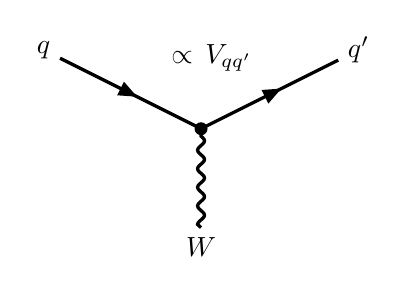
\begin{tikzpicture}
\begin{feynman}
    % Vertices
    \vertex (q)  at (0, 1.0) {$q$};
    \vertex[dot] (v)  at (2, 0) {};       
    \vertex (qp) at (4, 1.0) {$q'$};
    \vertex (W)  at (2,-1.5) {$W$};

    % Diagram
    \diagram*{
        (q)  -- [fermion, line width=1.2pt] (v) -- [fermion, line width=1.2pt] (qp),
        (v)  -- [boson, line width=1.2pt] (W),
    };

    % CKM label near the vertex
    \node[anchor=west] at (1.5,0.9) {$\propto\, V_{qq'}$};

\end{feynman}
\end{tikzpicture}
\end{document}
